\chapter{Dokumentace}

\section{Vstupní data}

\subsection{Struktura dat}

Jedná se o data ve formátu JSON, obsahující všechny potřebné informace o
rozložení nukleotidů, jejich párování, velikosti popisků, barvách a tlouštkách
čar. Kromě informací o rozložení lze z nich také vyčíst informace o potřebných
editacích vzorové sekundární struktury.

Každý nukleotid má svůj index a jméno (A, C, G nebo U). Kromě vlastního indexu
a jména je vedle uložené i jméno a index vzorového nukleotidu. Pokud se jedná o
přidaný nukleotid, index vzorového nukleotidu je $-1$. Za pomocí těchto
informací lze jednoduše zjistit, jestli je nukleotid přidaný nebo přejmenovaný
a pokud máme k dispozici i data vzorové struktury, lze pomocí indexu porovnávat
jejich souřadnice.

V rámci R2DT projektu vzníká JSON
schéma\footnote{https://github.com/LDWLab/RNA2D-data-schema}, které by mělo
popisovat strukturu vstupních dat. Schéma je stále ve vývoji, proto aktuální
výstupy Traveleru neodpovídájí schématu a je dost možné, že se formát výstupu
bude v budoucnu ještě měnit a naše knihovna se jim bude přizpůsobovat.

Samotná struktura dat není složitá, ale popíšeme zde pouze tu část, kterou
aktuálně využíváme, kromě toho, že ostatní data pro nás nejsou duležitá, tak
jak již bylo zmíněno samotná struktura dat není pevně daná a může se měnit.

Jedná se o objekt, který má dvě položky - \texttt{rnaComplexes} a
\texttt{classes}, což je pole objektů popisující třídy říkající způsob
zobrazení struktury, podobně jako to kaskádové
styly\footnote{https://developer.mozilla.org/en-US/docs/Web/CSS} (CSS) diktují
pro webové stránky. 

\texttt{rnaComplexes} je pole polí sloužící pro popis celých skupin RNA
struktur. Naše knihovna pracuje vždy pouze s nultým prvkem. Neviděli jsme důvod
to dělat jinak, a pokud by se nějaký důvod našel v budoucnu, neměl by být
problém naší knihovnu přizpůsobit situaci (např. rozšířením o novou metodu pro
zachování zpětné kompatibility).

V rámci naší knihovny jsme vytvořili interface, který vstupní data musí
splňovat. Struktura zbytku dat by měla být jasně viditelná z následujícího
diagramu těchto interfaceů.

\begin{figure}[H]
  \centering
  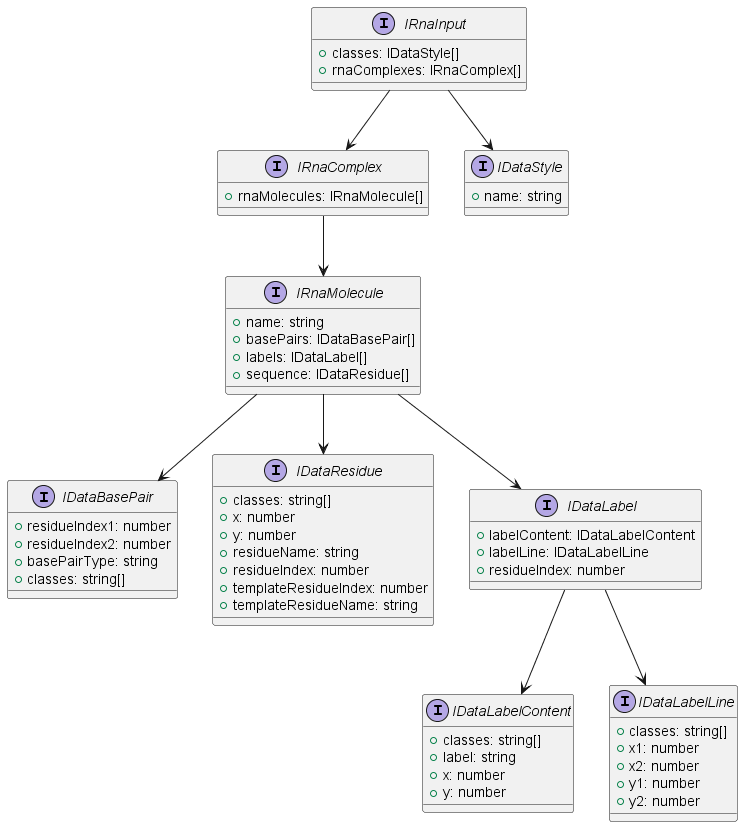
\includegraphics[width=145mm]{../img/kap03/rnaInput.png}
  \caption{Interface pro vstupní data.}
\end{figure}

\subsection{Získání vstupních dat}

RNACentral je otevřená databáze, která používá R2DT, ke generování rozložení
sekundárních RNA struktur. Pro přístup k databázi lze použít jak
API\footnote{https://rnacentral.org/api}, tak přímo posílat SQL
dotazy\footnote{https://rnacentral.org/help/public-database}.

Bohužel nezpřístupňuje mapování nukletidů na vzorovou strukturu, přesto je
databáze užitečná pro získání vstupních dat, protože obsahuje struktury a ke
každé takové struktuře informaci, ze které byla vygenerovaná. 

Pro získání testovacích dat jsme využívali veřejný SQL přístup\footnote{Použitý
dotaz: https://gist.github.com/davidhoksza/52df5b0fa5d85fdc4513966d2b50792b}.
Vybrali jsme nějaké vzorové struktury různého typu, ke každému jsme vybrali
náhodně nejvýše $20$ RNA molekul, které použili danou vzorovou strukturu pro
generování. Následně jsem použili R2DT, které jsme řekli, jakou vzorovou
strukturu použít pro vygenerování vstupních dat.

\section{Objektový návrh}

V následující části se pokusíme čtenáře seznámit s objektovým návrhem naší
knihovny. V této části dáme obecný pohled na strukturu tříd a později i ukážeme
jak se s třídama dá pracovat.

Srdcem celé knihovny je třída \texttt{RnaVis}. Má v sobě uložené vrstvy
realizované třídou \texttt{Layer}, představující jednotlivé struktury. Třída
\texttt{RnaVis} vykresluje struktury na canvas, nastavuje se přes ní
zoom/posouvání a zpřístupňuje většinu funkcionality.

Pro určení vykreslovacích parametrů (např. font, barva, velikost) objektů  máme
třídu \texttt{Styles}. Před každým vykreslením se zeptáme této třídy na
vykreslovací parametry pro daný objekt. Důvod, proč jsme zvolili takovéhle
řešení problému je, že jsme původně neměli jasnou představu, co a jak bude
řešené, a proto nám příšlo nejjednoduší tuto část oddělit a použít stejný
způsob, jaký se používá ve vstupních datech.

Poslední důležitou velkou částí jsou animace. Tuto funkcionalitu zpřístupňují
dvě hlavní třídy - \texttt{TranslationAnim}, \texttt{VisibilityAnim}. Obě
implementují interface \texttt{IAnimation}. 

Níže jsou tři diagramy tříd, které dohromady obsahují každou třídu. Diagramama
se snažíme vyjádřit obecnou strukturu, tím pádem pro přehlednost neobsahují
všechny informace - všechny metody, některé privátní vlastnosti a některé
závislosti. Pro podrobnější rozbor tříd a metod se doporučujeme podívat do
referenční
dokumentace\footnote{https://github.com/michalhercik/rna-visualizer/blob/main/lib/docs/README.md}.
 
\begin{figure}[H]
  \centering
  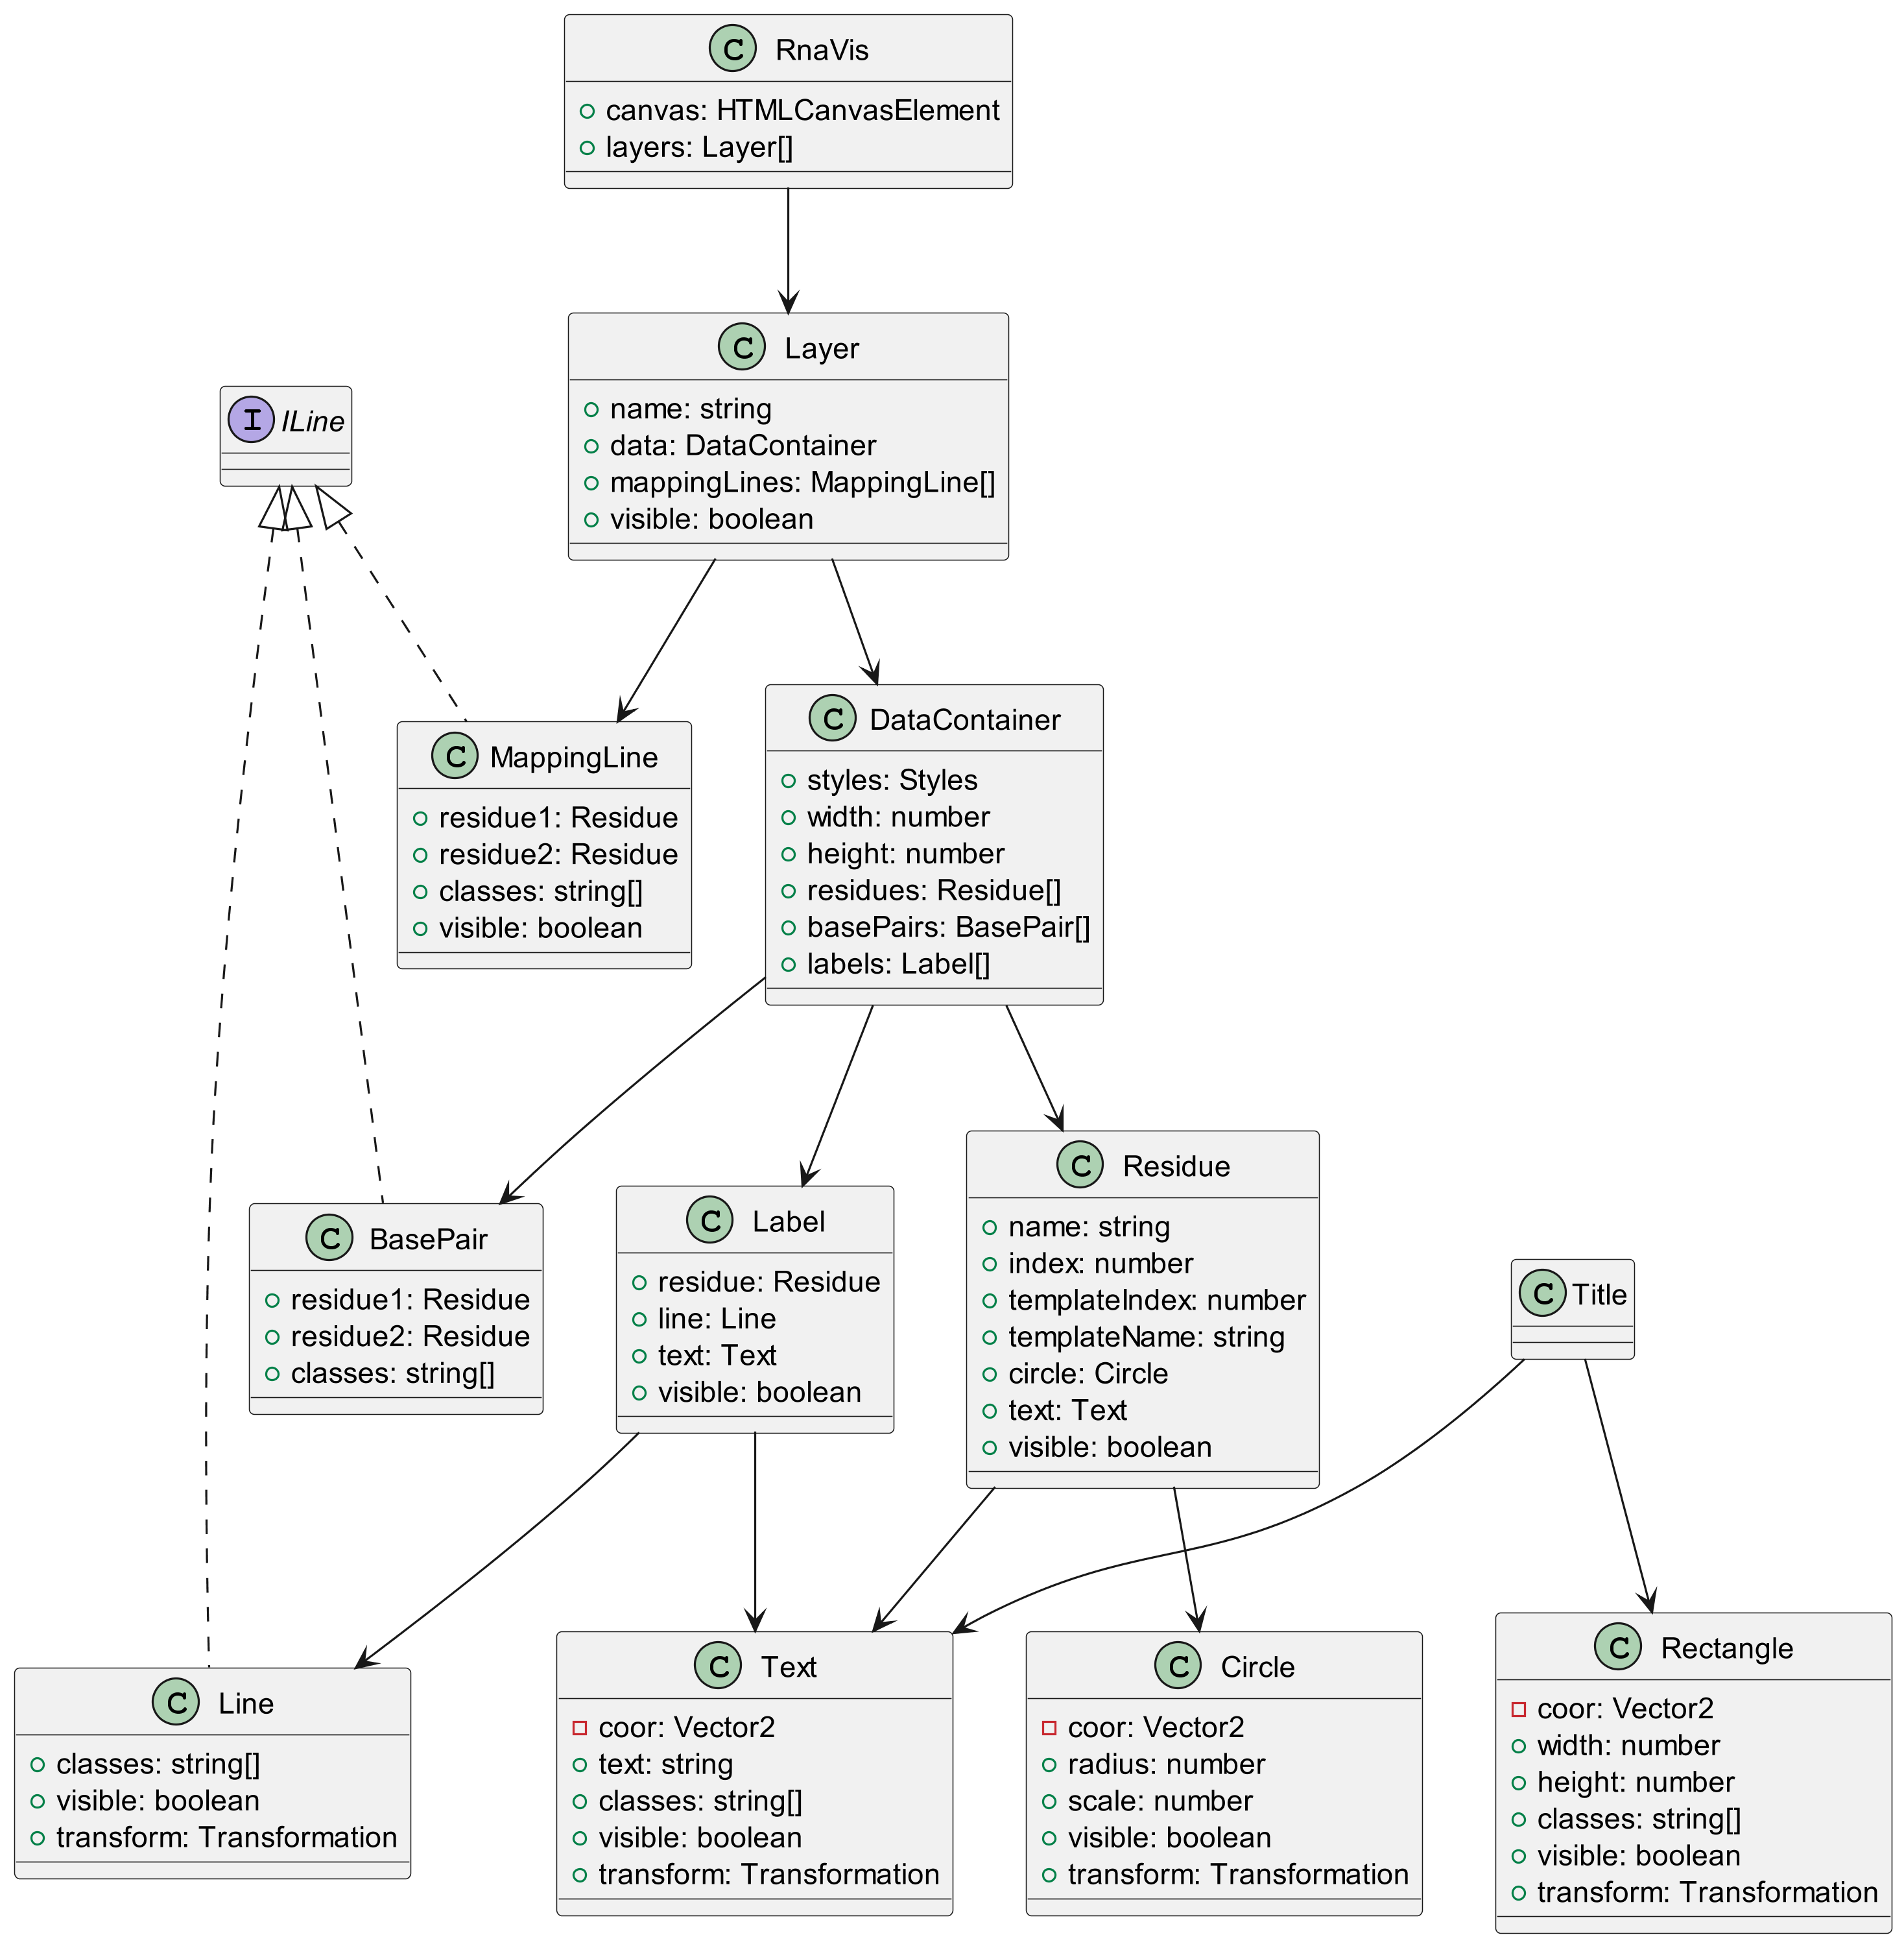
\includegraphics[width=145mm]{../img/kap03/rnavis.png}
  \caption{Diagram tříd.}
\end{figure}

\begin{figure}[H]
  \centering
  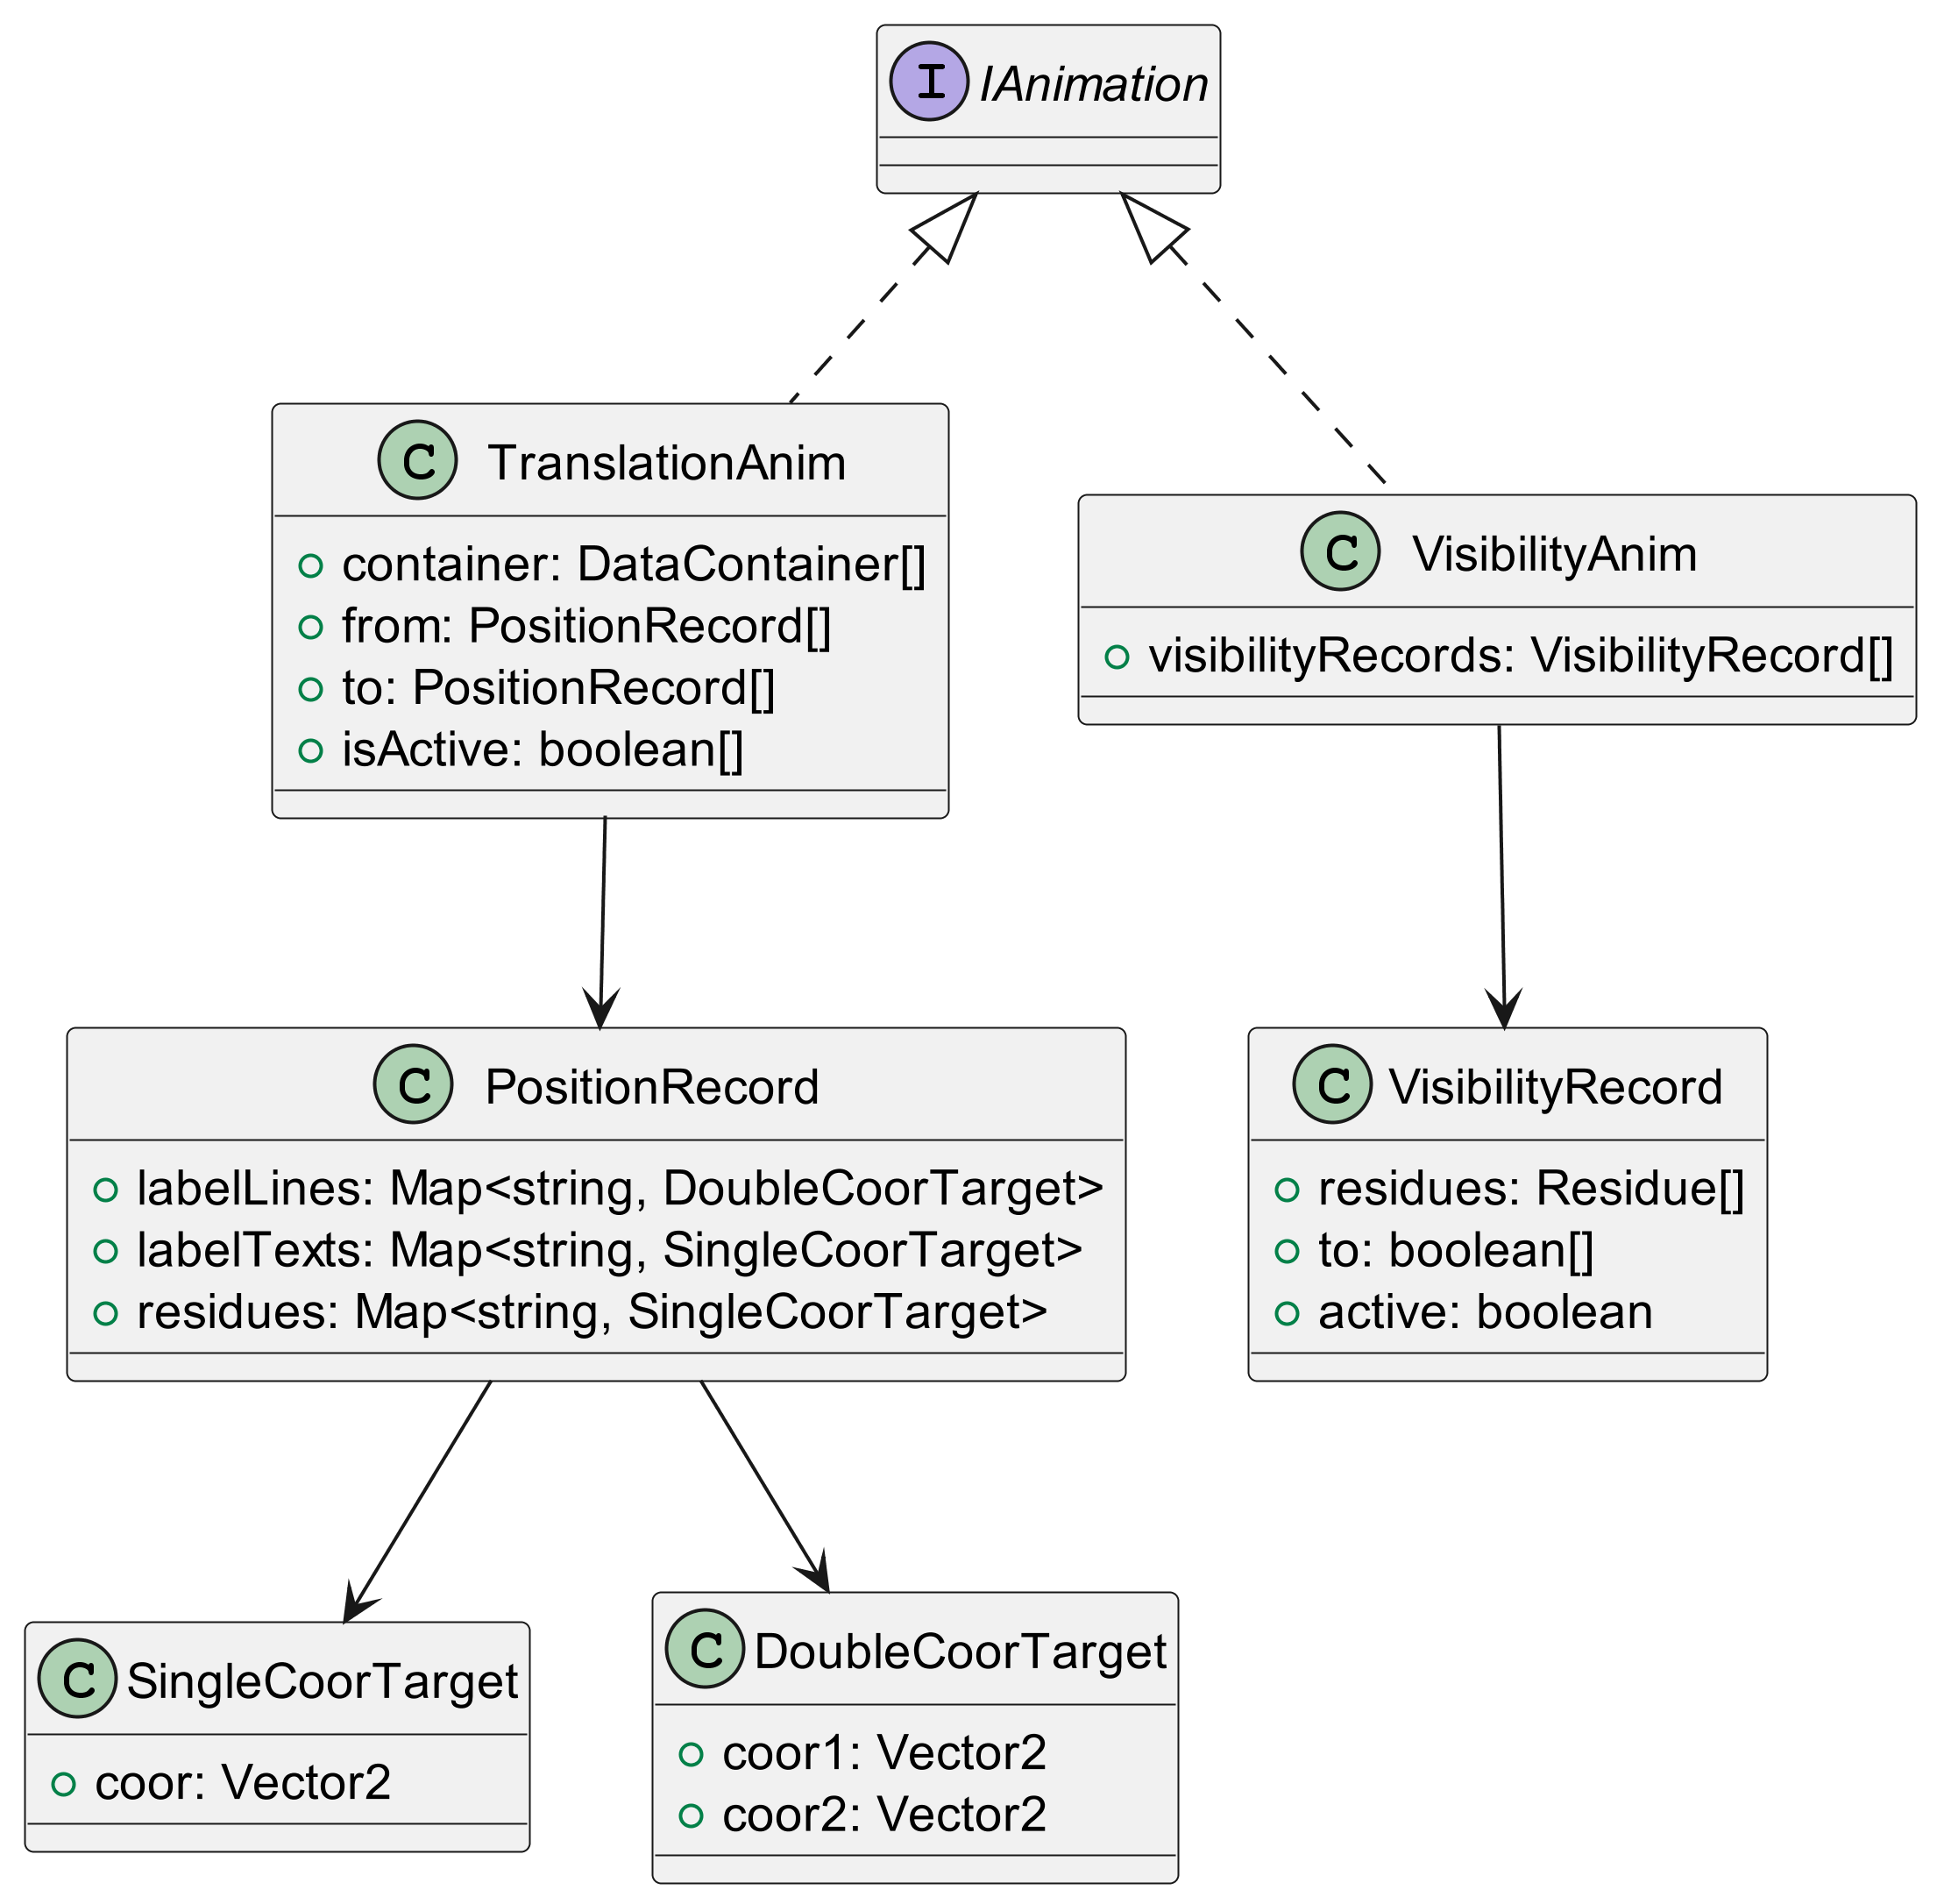
\includegraphics[width=145mm]{../img/kap03/animation.png}
  \caption{Diagram tříd.}
\end{figure}

\begin{figure}[H]
  \centering
  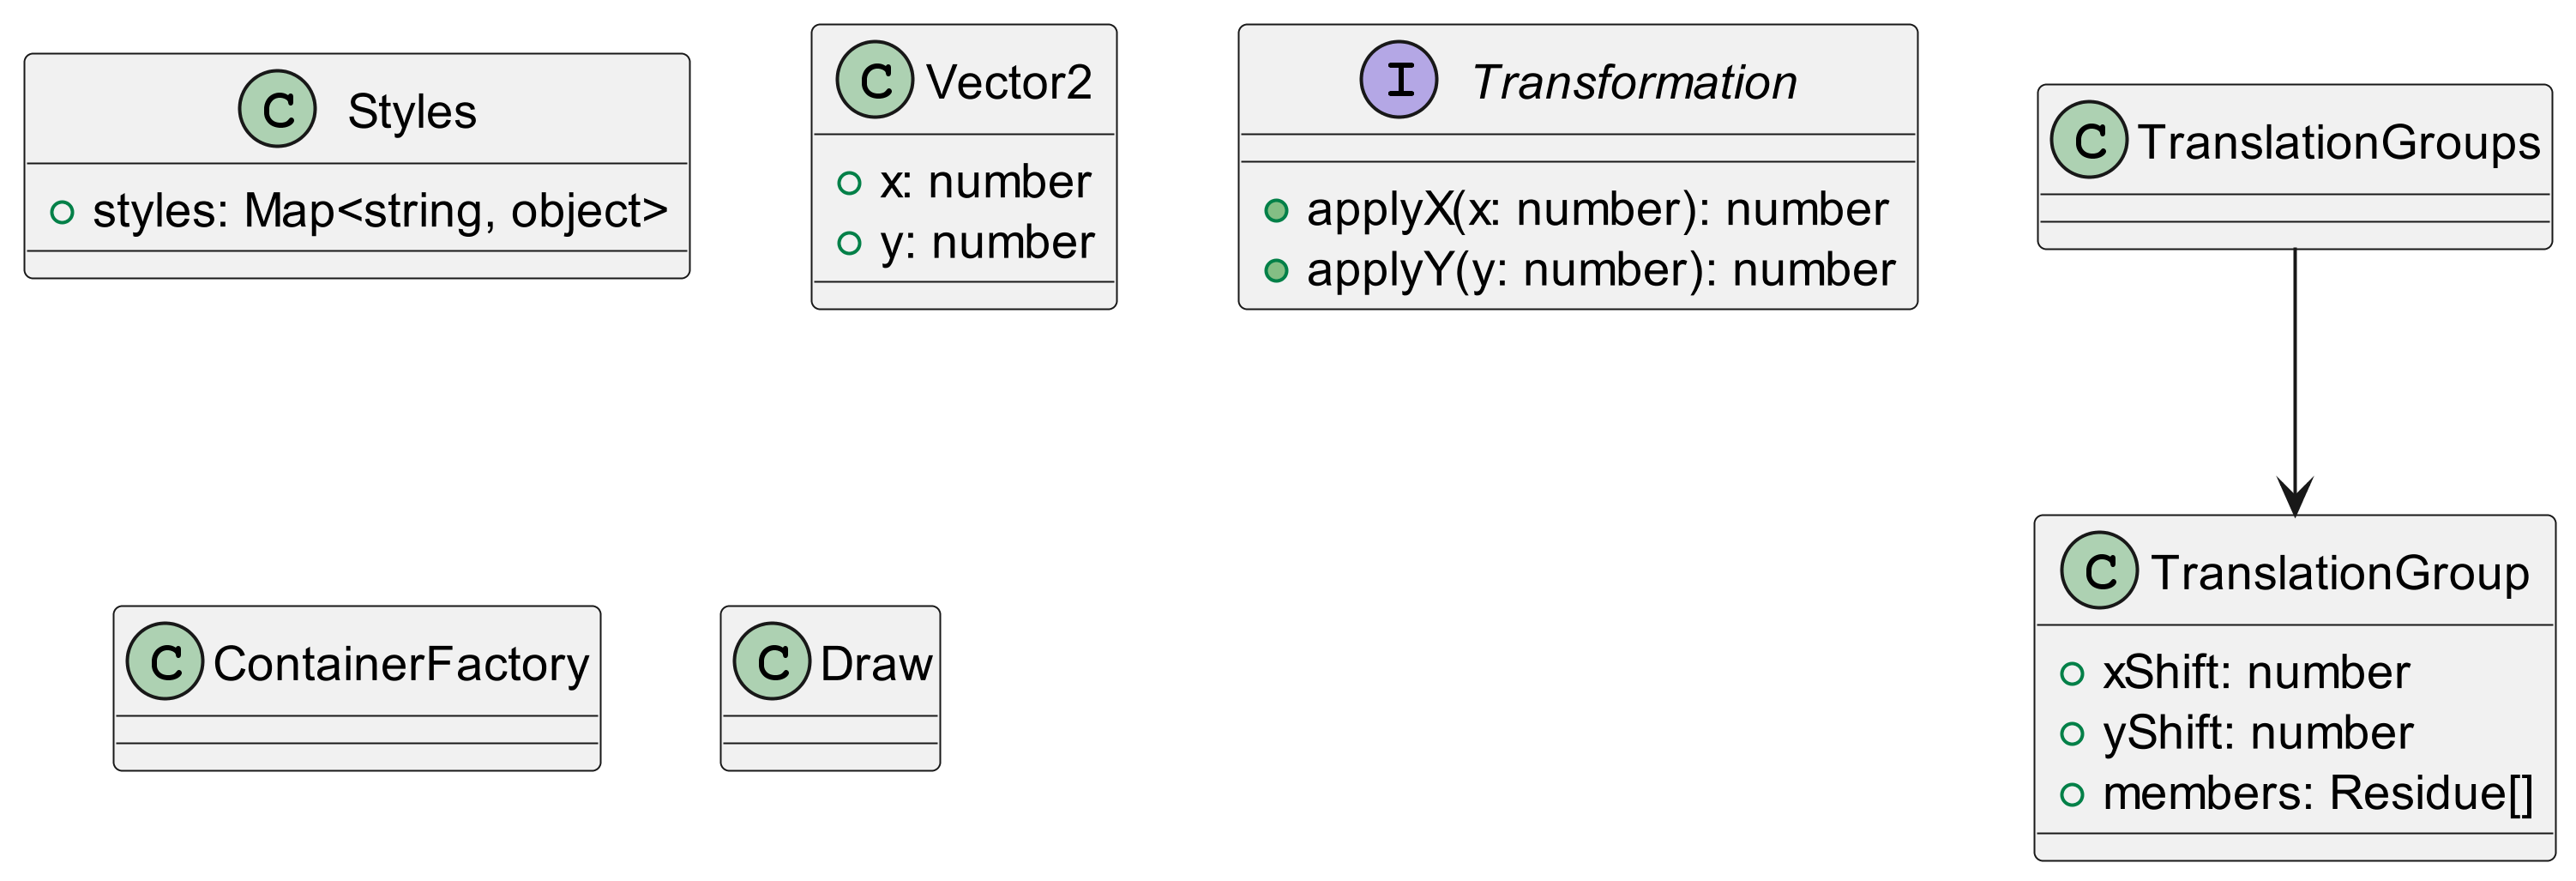
\includegraphics[width=145mm]{../img/kap03/others.png}
  \caption{Diagram tříd.}
\end{figure}

\section{Uživatelské seznámení s knihovnou}

S obecnou strukturou kódu jsme čtenáře seznámili a nyní se pokusíme ukázat, jak
lze knihovnu užívat. Bude se jednat o ukázku implementací základních využití,
jako je vykreslení struktur, zarovnání, transformace na vzorovu strukturu a
některé další možnosti.

\subsection{Vytvoření objektu RnaVis a vykreslení struktur}

V prvním kroce importujeme veškeré potřebné zdroje. Pužité vstupní data
\texttt{d.5.b.A.madurae.json} a \texttt{URS00000B9D9D.json} jsou dostupné na
GitHub stránce
projektu\footnote{https://github.com/michalhercik/rna-visualizer/blob/main/demo/example\_data/madurae\\/URS00000B9D9D\_471852-d.5.b.A.madurae.json}
\footnote{https://github.com/michalhercik/rna-visualizer/blob/main/demo/example\_data/madurae\\/d.5.b.A.madurae\_fromn\_d.5.b.A.madurae.colored.json}

\begin{code}
import { 
  RnaVis, 
  TranslationGroups, 
  PositionRecord,
  TranslationAnim,
} from 'rna-visualizer';
import template from './d.5.b.A.madurae.json';
import structure from './URS00000B9D9D.json';
\end{code}

Následně vytvoříme \texttt{canvas}, na který budeme vykreslovat, nastavíme mu
šířku, výšku a přidáme ho do těla dokumentu.

\begin{code}
const canvas = document.createElement('canvas');
canvas.width = 500;
canvas.height = 500;
document.body.appendChild(canvas);
\end{code}

Nyní už můžeme vytvořit samotný objekt \texttt{RnaVis}, který nás bude provázet
v ostatních ukázkách.

\begin{code}
const rnaVis = new RnaVis(canvas);
\end{code}

Přidáme do něj dvě struktury - \texttt{template} a \texttt{structure}.
Struktury se přidávají pomocí metody \texttt{addLayer}, která má tři parametry
- přidávanou strukturu, libovolný název a poslední třetí parametr je volitelný
a slouží k určení, jestli chceme, aby se struktura vykreslovala a jeho
defaultní hodnota je \texttt{true}, tedy defaultně se struktura vykresluje.
Knihovna předpokládá, že první přidaná struktura, je vzorová struktura, ze
které jsou všechny ostatní vygenerované.

\begin{code}
rnaVis
  .addLayer(template, 'd.5.b.A.madurae')
  .addLayer(structure, 'URS00000B9D9D');
\end{code}

Struktury lze potom vykreslit pomocí metody \texttt{draw}.

\begin{code}
rnaVis.draw();
\end{code}

Celý kód lze zapsat následovně.

\begin{code}
import { 
  RnaVis, 
  TranslationGroups, 
  PositionRecord,
  TranslationAnim,
} from 'rna-visualizer';
import template from './d.5.b.A.madurae.json';
import structure from './URS00000B9D9D.json';

const canvas = document.createElement('canvas');
canvas.width = 500;
canvas.height = 500;
document.body.appendChild(canvas);

new RnaVis(canvas)
  .addLayer(template, 'd.5.b.A.madurae')
  .addLayer(structure, 'URS00000B9D9D')
  .draw();
\end{code}

V dalších ukázkách budeme předpokládat předchozí kroky a budeme na ně
navazovat.

\subsection{Zoom a posouvání canvasu}

Pro zoom a posouvání používáme d3.js knihovnu. Není ale třeba používat jejich
rozhraní, protože třída \texttt{RnaVis} obsahuje metodu \texttt{addZoom}, která
přidá jak zoom tak posouvání canvasu.

\begin{code}
rnaVis.addZoom();
\end{code}

\subsection{Zarovnání struktur}

Zarovnání struktur docílíme tak, že zavoláme na instanci třídy \texttt{RnaVis}
metodu \texttt{align}, která vrátí pole objektů typu \texttt{Vector2}, které
reprezentují posunutí pro každou strukturu. Následně zavoláme na instanci třídy
\texttt{RnaVis} metodu \texttt{translate}, které předáme pole obsahující
posunutí a metoda posune každou strukturu o příslušné posunutí. Potom už stačí pouze vykreslit struktury metodou \texttt{draw}.

\begin{code}
const translations = rnaVis.align();
rnaVis
  .translate(translations);
  .draw();
\end{code}

\subsubsection{Zarovnání struktur na konkrétní skupinu}

Metoda \texttt{align} má volitelný parametr typu \texttt{number}, kterým můžeme
vybrat, na kterou skupinu nukleotidů chceme dostat zarovnání.

Při první iteraci se porovnává první přidaná struktura (vzorová) s druhou
přidanou strukturou a roztřídí se nukleotidy podle posunutí, které je zarovná.
Číselný parametr potom určuje, která skupina se použije pro filtrování v
dalších iterací. 

Pokud je parametr prázdný nebo menší než nula, vybere se největší skupina.
Pokud je parametr větší, než počet vytvořených skupin metoda vyhodí vyjímku se
zprávou \texttt{groupIndex >= groups.length}. 

V následující ukázce vytvoříme skupiny, které vzniknout při první iteraci a
vybereme nejmenší, kterou pak použijeme pro zarovnání struktur. Skupiny
vytvoříme statickou metodou \texttt{TranslationGroups.create}. První parametr
je vzorová struktura, druhý parametr je struktura, kterou chceme zarovnat.
Třetí parametr jsou skupiny pomocí, kterých chceme filtrovat a je volitelný a
poslední parametr je minimální velikost výstupních skupin, který je taky
volitelný a jeho defaultní hodnota je $5$.

\begin{code}
const containers = rnaVis.getDataContainers();
const groupSizes = 
  TranslationGroups.create(containers[0], containers[1], null, 20)
  .map(group => group.size());
const groupIndex = groupSizes.indexOf(Math.min(...groupSizes));
const translationsToGroup = rnaVis.align(groupIndex);
rnaVis
  .translate(translationsToGroup)
  .draw();
\end{code}

\subsubsection{Zarovnání na nukleotid}

Zarovnání na nukletodi obsahuje podobné kroky. Nejdřív si zvolíme nukleotid ze
vzorové struktury, na který chceme struktury zarovnávat. Potom na instanci
třídy \texttt{RnaVis} pomocí metody \texttt{getAlignmentToTempResidue} získáme
posunutí pro každou strukturu a nakonec struktury zarovnáme a vykreslíme.

\begin{code}
const templateResidue = rnaVis.layers[0].data.residues[42];
const translationsToResidue = 
  rnaVis.getAlignmentToTempResidue(templateResidue);
rnaVis
  .translate(translationsToResidue)
  .draw();
\end{code}

\subsubsection{Animace zarovnání}

Jakýkoliv přechod je pro oko vždy příjemnější animovat a to knihovna umožňuje
pomocí jednoduchého rozhraní pro animace. V následující ukázce ukážeme jak
animovat zarovnání struktur.

V prvním kroce vytvoříme pro každou strukturu \texttt{PositionRecord}, který
obsahuje pozice nukleotidů a popisků. V tomto případě bude obsahovat cílovou
pozici pro každý nukleotid a vytvoříme ho pomocí statické metody
\texttt{fromTranslation}, která bere jako parametr strukturu a posunutí
struktury.

Následně vytvoříme objekt typu \texttt{TranslationAnim}, který umožňuje mimo
jiné animovat transformaci struktury na daný \texttt{PositionRecord}. Potom už
jenom zavoláme metodu \texttt{animate}, kterou začné celá animace. Jako
parametry bere instanci třídy \texttt{RnaVis}, kterou používá pro vykreslování
každého snímku animace, trvání animace v milisekundách a poslední volitelný
parametr je funkce, která se zavolá na konci animace. V ukázce na konci animace
jí otočíme a animujeme zpátky do původního stavu.

\begin{code}
const containers = rnaVis.getDataContainers();
const animationTargets = rnaVis
  .align()
  .map((translation, i) 
    => PositionRecord.fromTranslation(containers[i], translation)
  );

const anim = new TranslationAnim(containers, animationTargets);
anim.animate(rnaVis, 1500, () => {
  anim.reverse();
  anim.animate(rnaVis, 1500);
});
\end{code}

\subsection{Mapovací čáry}

Zobrazení čar, které ukazují mapování nukleotidů, je velmi jednoduché.
Mapovací čáry se vytvoří hned při přidání každé vrstvy a jsou defaultně
schované, proto je stačí pouze zviditelnit.

\begin{code}
rnaVis.layers.forEach(
  l => l.mappingLines.forEach(
    m => m.setVisible(true)
  )
);
rnaVis.draw();
\end{code}

\subsection{Transformace na vzorovou strukturu}

Poslední ukázkou je transformace na vzorovou strukturu. V ukázce nejdříve
schováme nukleotidy, které nemají vzorový nukleotid. Potom vytvoříme opět
\texttt{PositionRecord}, tentokrát pomocí statické metody
\texttt{fromTemplate}, která každýmu nukleotidu dá pozici jeho vzorového
nukleotidu. Potom už jenom animujeme přechod.

\begin{code}
const containers = rnaVis.getDataContainers().slice(1);
const targetStructure = rnaVis.layers[0].data;

containers.forEach(c => {
  c.getUnmappableResidues().forEach(
    r => r.setVisible(false)
  );
});

const targets = containers.map(
  cont => PositionRecord.fromTemplate(cont, targetStructure)
);
new TranslationAnim(containers, targets)
  .animate(rnaVis, 1500);
\end{code}

\section{Použití canvasu}

\subsection{Knihovna D3.js}

D3.js\footnote{https://d3js.org/} je knihovna v jayzce Javascript pomáhající
přivést data k životu podporující především
SVG\footnote{https://developer.mozilla.org/en-US/docs/Web/SVG}. SVG je webový
standard, který lze skvěle kombinovat s ostatními standardy jako je CSS,
DOM\footnote{https://developer.mozilla.org/en-US/docs/Web/API/Document\_Object\_Model},
Javascript.

D3.js knihovna klade důraz na webové standardy a tím dává uživateli možnost
využívat moderní prohlížeče naplno bez dalších frameworků. S knihovnou není
nejjednodušší se naučit pracovat, ale její velkou předností je rychlost a
široká paleta funkcí pro vizualizace dat.

\subsection{SVG}

V počátcích jsme chtěli k zobrazování používat SVG, které V kombinací s D3.js
knihovnou je velmi silný a flexibilní nástroj.

Bohužel SVG je poměrně pomalé a je to poznat už při vykreslování tisícovek
objektů. Takového počtu objektů můžeme dosáhnout pouze s jednou sekundární RNA
strukturou, my navíc chceme zobrazit více takových struktur a ještě s nimi
dynamicky pracovat. Tím se pro nás stalo SVG nepoužitelné.

\subsection{Canvas}

Další možností bylo využití
canvasu\footnote{https://developer.mozilla.org/en-US/docs/Web/API/Canvas\_API},
který slibuje výrazně lepší výkon a lze ho stále jednoduše používat.

Některé pro nás klíčové funkce D3.js knihovny lze využít i pro práci s
canvasem. Konkrétně se jedná o zoom, posouvání a animace.

U canvasu jsme nakonec i zůstali, přestože při práci s desítkama velkých
struktur vykreslování není plynulé.

\section{Demonstrace metod}

V rámci naší knihovny jsme vytvořili také webovou
aplikaci\footnote{https://michalhercik.github.io/rna-visualizer/}, která
demonstruje možnosti naší knihovny. Tato aplikace umožňuje uživatelům pracovat
s jednotlivými metodami nebo se všemi metodami najednou pro usnadnění porovnání
- překládání se zarovnáním, transformace na vzorovou strukturu, mapovací čáry a
další možnosti pro zpříjemnění práce. 

\begin{figure}[H]
  \centering
  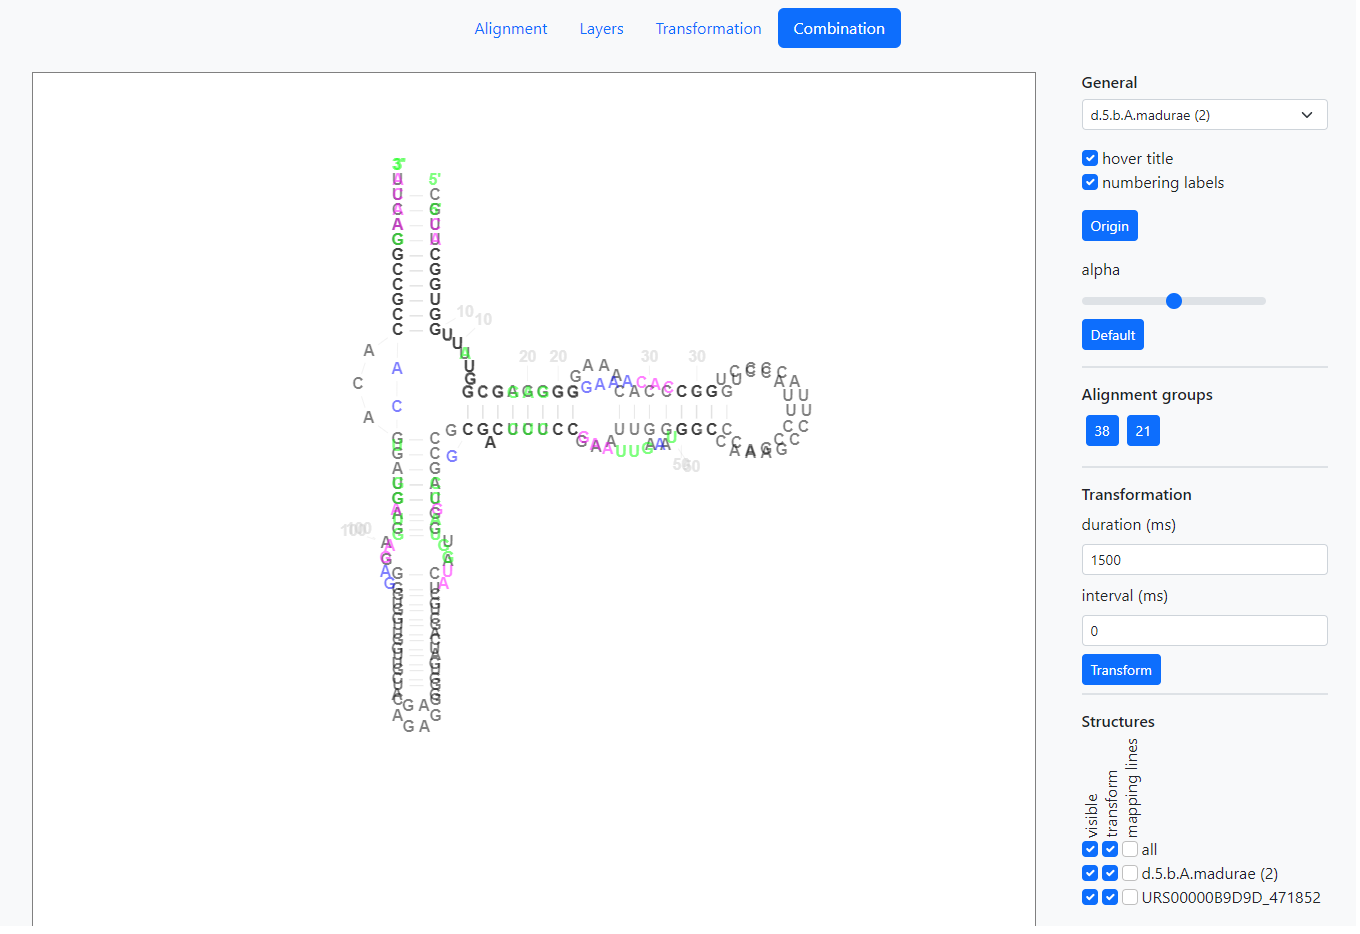
\includegraphics[width=145mm]{../img/kap03/demo.png}
  \caption{Screenshot aplikace vytvořené pro demostraci funkcionality knihovny.}
\end{figure}
